\documentclass{article}
\pagenumbering{gobble}
\usepackage{amsmath}
\usepackage{amsfonts}
\usepackage{amssymb}
\usepackage{graphicx}
\usepackage[T2A]{fontenc}
\usepackage[utf8]{inputenc}
\usepackage[russian,english]{babel}
\newtheorem{theorem}{Теорема}[section] % Теоремы нумеруются внутри главы
\newtheorem{theorem*}{Теорема}
\newtheorem{corollary}{Следствие}
\newtheorem{lemma}{Лемма}
\newtheorem{case}{Случай}[theorem]
\newtheorem{definition}{Определение}
\begin{document}
\title{Теория трансляции, \\(Кампилятторы)}
\selectlanguage{russian}
\maketitle
\newpage
    \section{Что то}
    в стековых методах используется стеки и таблица переходов,
    для того чтобы правильно заполнить таблицу переходов. 
    При считывании операндов переходов
    при считывании $i$ 
    
    В таблцие переходов указывется какие едействия должен выполнять транслятор и в этой таблице каждой операции языка соответсвует строка и столбец.
    Переменными таблицы являются директивы транслятора, реализуемые в виде вожможных 4-х действий транслятора.
    Действия выполняются после считывания
    Операции в вершине всека - $\theta$
    \begin{itemize}
        \item Заслать $\theta$ в T и читать след символ
        \item Генерировать Kn, заслать $\theta$ в T, читать след символ
        \item Читать из T, читать след символ (используется для удаления скобок)
        \item Генерировать Kn, читать из T, повторить с тем же входным символом
    \end{itemize}
    В таблице выделены специаль\dots \\
    Процессор выбирает в качестве входного символа верхнюю операцию в качестве входного что?
    А $Ksi$ - последней\dots
    $\Lambda$ - пробел или пустая строка, \\
    Т.О. \\
    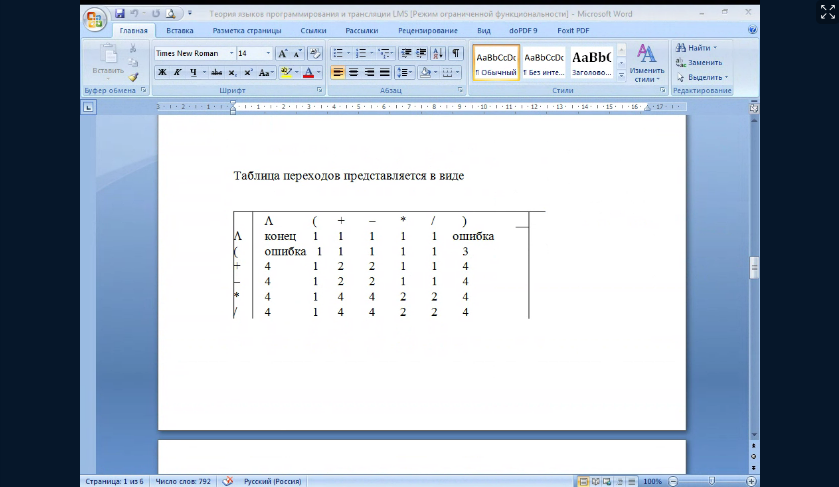
\includegraphics[scale=0.5]{../pictures/1.png}
    \begin{table}
        
    \end{table}
    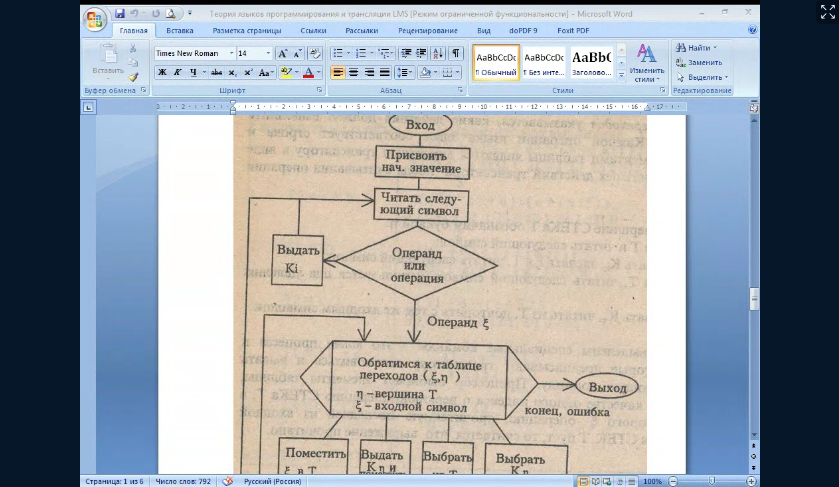
\includegraphics[scale=0.5]{../pictures/2.png}
    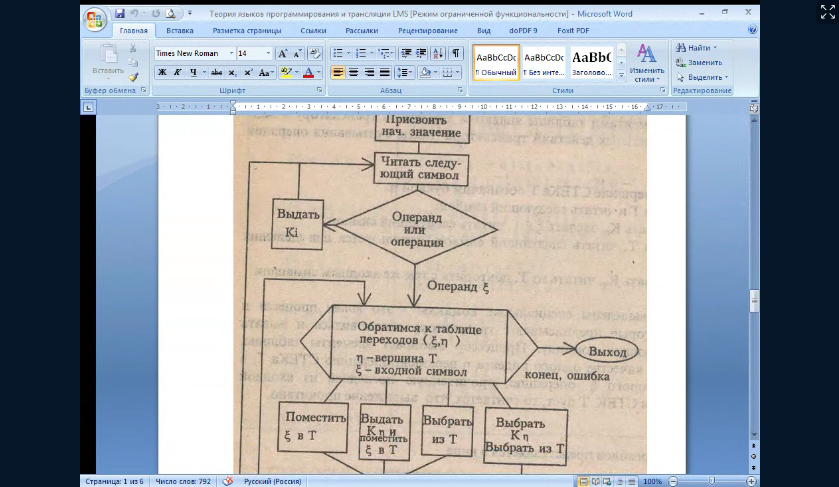
\includegraphics[scale=0.5]{../pictures/3.png}
    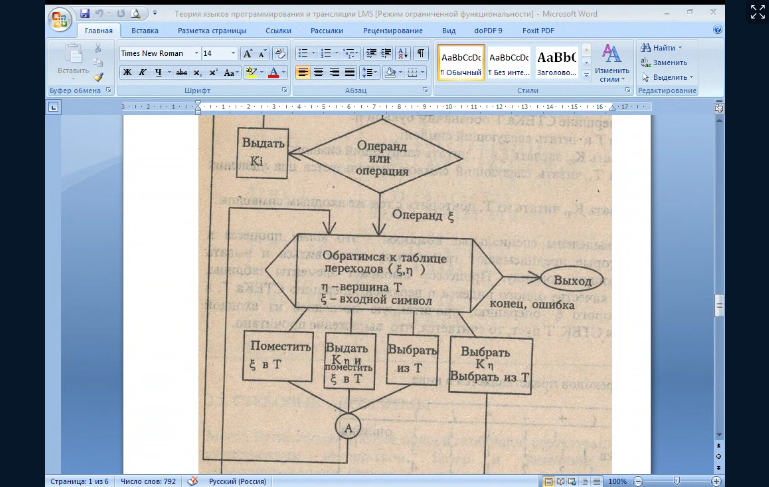
\includegraphics[scale=0.5]{../pictures/4.png}

    Рассмотрим выражение: $(a*b+c*d)/(a-d)+b*c$ \\

    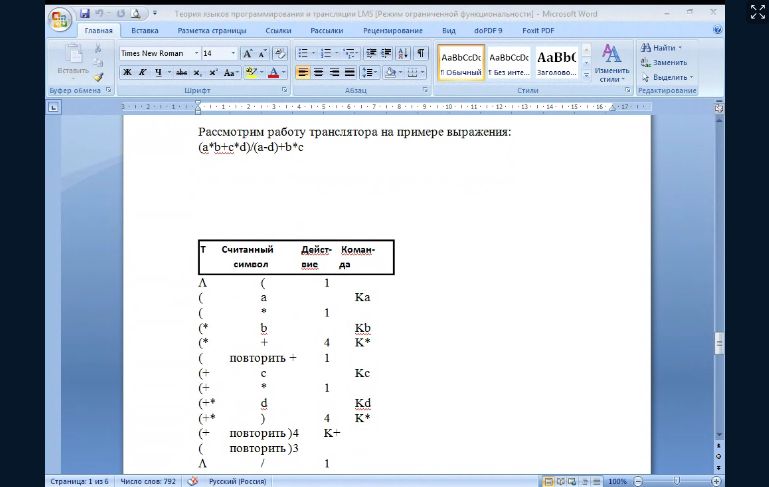
\includegraphics[scale=0.5]{../pictures/5.png}
    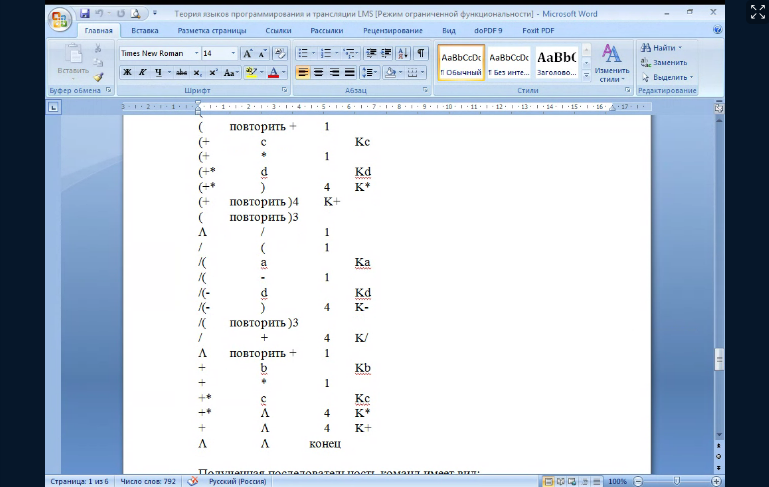
\includegraphics[scale=0.5]{../pictures/6.png}
    Полученна последоввательность комманд:
    $$
       Ka, Kb, K*, Kc, Kd, K*, K+, Ka, Kd, K-, Kb, Kc, K*, K+
    $$
    Опустив K, получим: $ab*cd*+ad-/bc*$
    Получена обратная Польская запись

    Исполнающая программа использует стек Е и читает польскую запись слева направо.
    Дальше при чтении операнда он засылается в стек Е, а при чтении операции она применяется к двум верхним элементам Е.
    Для записи выдаваемой транслятором не возникает явных или неявных ппроблем старшинства операций.
    Т.е. программа выполняется слева направо.
    Временная память автоматически управляется стеком Е, а она содержит все времменые промежуточные значения.
\newpage
    \section{Формальные модели грамматик}


\end{document}